\documentclass{article}

\usepackage{hyperref}
\usepackage{parskip}
\usepackage{amsthm}
\usepackage{amsmath}
\usepackage{amssymb}
\usepackage{wrapfig}
\usepackage{graphicx}
\usepackage{listings}
\usepackage{color}
\usepackage{fullpage}
\newcommand{\code}{\texttt}

\author{Micah Wylde\\Jeffrey Ruberg}
\date{\today}
\title{Autonomous Agents:\\
A Hybrid Dynamical System for Vehicle Navigation\\
Comp 352}

\begin{document}
\maketitle

\section{Introduction}
Self-driving cars hold much promise for saving fuel, time and
lives. Human-driven vehicles are responsible for millions of traffic accidents
and over 30,000 deaths annually in the US alone. Humans can also make poor
decisions in regards to routes, leading to traffic jams and wasted fuel. Safe,
effective autonomous cars could largely solve these issues. AI researchers have
been interested in the potential for vehicular navigation since the 1960s. In
order to spur development in this area, the Defense Advanced Research Projects
Agency (DARPA) organized the Grand Challenge in 2004, which tasked contestants
to build cars which could autonomously navigate a 142 mile-long course in the
Mojave desert. Though none of the vehicles could finish the course, a second
competition the next year was more successful. Four teams finished in the
allotted time, traversing a treacherous 132 mile desert course with no human
guidance. Building on this achievement, in 2007 DARPA organized the Urban
Challenge which took place in a simulated suburban environment. To win, cars had
to navigate a maze of streets while accounting for other traffic and following
California traffic laws at all times. Six teams finished the 61 mile course with
the winner, ``Boss'' from CMU, taking a little more than four hours
\cite{robotic_cars}.

There are many challenges involved in autonomous driving and robot navigation in
general. In the real world one must deal with unreliable and imperfect sensor
data, imprecise localization technologies and other perception issues. Even in
simulation the challenges of successful navigation are immense. Cars must follow
traffic laws, get to their destination quickly and efficiently and act safely at
all times, even in unexpected situations. As far as the actual navigation, there
are two general approaches: deliberative and reactive. As an example of the
former, $A^*$ is an efficient and optimal graph search algorithm which is very
effective at finding the best route between two points but cannot handle the
dynamism of the real world. Dynamical systems-based navigation is a reactive
strategy that uses force fields to guide agents away from obstacles and towards
their target. However, it is purely local and has trouble finding optimal paths
to distant goals. In this paper we present simulated agents which use each
technique as well as a hybrid agent which makes use of $A^*$ for global
navigation and dynamical systems for local navigation.


\section{Autonomous Driving}

\subsection{Simulation}

\section{Methods}

To create an autonomous agent that navigates while simulating a car's behavior
and traffic laws, we took three general approaches: deliberative planning
through $A^*$ search, reactive navigation through a dynamical system, and a
hybrid of deliberative planning and reactive motion. The system architecture
consists of a server and a separate client for each agent.

\subsection{System Architecture}

The project is written in Ruby, specifically JRuby\footnote{JRuby is an
  implementation of the Ruby Programming Language on top of the Java Virtual
  Machine, which allows integration between Java and Ruby code} to utilize
Java2D for the graphical display. As a result, the server code runs solely under
JRuby, but client code can additionally be run using Ruby 1.9. Agents are
represented both on the client and server end; server agents perform motion and
display-related calculations, and client agents contain all the navigation
inference and decision-making and ultimately send decisions (restricted to
behavior variables) back to the server again.

\begin{figure}[h]
  \begin{center}
    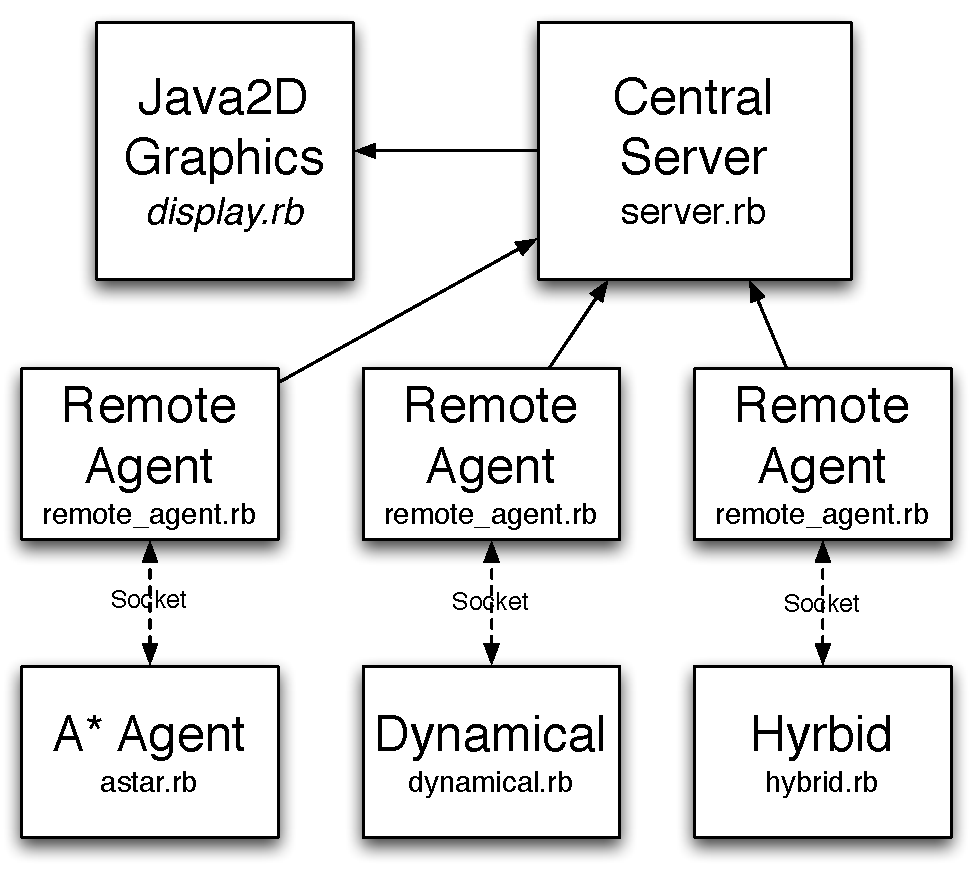
\includegraphics[width=0.5\textwidth]{architecture}
  \end{center}
  \caption{The system architecture of the simulation. Solid lines connect
    components included in the same process, while dotted lines indicated socket
    connections between discrete processes.}
  \label{architecture}
\end{figure}

A brief description of the roles of the various source files will follow.

\begin{description}
\item[app.rb] The point of entry for the program. Processes
  command-line options and can optionally start a server, start a new
  agent, or run tests.

\item[client\_agent.rb] Contains the \code{ClientAgent} class, the
  super class which every client agent inherits. Client agents receive
  messages from remote server agents, process the message (based on
  their form of navigation), and then send back a response in their
  behavior variable space.

\item[constants.rb] Contains various general constants that may be
  used in several locations or files, or that may be particularly useful to
  tweak with.

\item[display.rb] Contains all of the display code used to generate
  our rendering of the world.

\item[map.rb] Contains the classes, specifically \code{Map}, which
  encode information provided from real map data.

\item[pqueue.rb] A priority queue implementation used for $A^*$ search.

\item[remote\_agent.rb] Contains the \code{RemoteServerAgent} class,
  which is a subclass of \code{ServerAgent}. Essentially, a remote
  server agent is a server agent which is tied to a specific client
  agent and communicates with that client agent.

\item[server\_agent.rb] Contains the \code{ServerAgent} class, which
  contains all the base representation and calculations needed for an agent (for
  example, the server agent computes various points needed to display the agent
  graphically).

\item[server.rb] Contains the socket server which handles agent connections.

\item[socket.rb] Contains code for handling communication between
  clients and the server

\item[util.rb] Contains a collection of geometry classes
  (\code{Point}, \code{Vector}, etc.) which are useful in the display
  and other various places (most notably in dynamical navigation
  calculations).

\item[agents/astar.rb] Contains a client agent that deliberatively
  plans paths using $A^*$ search.

\item[agents/dynamical.rb] Contains a client agent that navigates
  through a purely dynamical system-based approach.

\item[agents/hybrid.rb] Contains a client agent that navigates through
  a combination of deliberative planning and dynamical systems.

\item[agents/simple.rb] Contains a very primitive client agent (that
  can hardly be called an agent) which allows us to easily test the
  motion calculations performed by server agents.

\end{description}

\subsection{Simulation}
To provide a realistic environment for navigation tests, we used real-world map
data from OpenStreetMap.org, which provides XML-formatted maps for the entire
world. The data format, called OSM, provides a graph representation of a road
system; streets are represented by placing nodes wherever the road turns or
intersects other roads, with edges connecting each node. To provide testing
data, we used the website to export maps of Hayward, CA and Santa Cruz, CA. We
wrote a program, \code{osm\_convert}, which converts an OSM XML file to a
YAML\footnote{YAML (a recursive acronym for YAML Ain't Markup Language) is a
  language-independent data serialization standard which allows easy conversion
  of data structures to and from a string representation.} format. In
\code{map.rb} we then read this YAML data and construct an internal
representation of the graph, converting points specified by latitude and
longitude to a scale of meters.

In order to make an internal representation of the map suitable for a driving
simulation, we generate a \emph{road} for each graph edge by creating
\emph{walls} (belonging to the \emph{road}) defined as parallel lines a constant
\code{ROAD\_WIDTH} away from the center line, which is the line connecting the
node and the node the edge connects it to. This parallel line approach creates
overlapping walls at every acute angle and gaps at every obtuse angle, so we
process the \emph{walls} to clip them where they overlap and extend them where
they leave gaps.

To run the display, we start a server by running the script \code{bin/driving}
without any command line arguments (or with arguments to specify window geometry
or map file). The display renders the world by drawing every \emph{road} as a
polygon with points defined by its \emph{walls}. In the display, we have
implemented mouse dragging, zooming, pausing, agent centering (on by default,
toggled with space bar), and agent dragging.

To create an agent, we create an agent process (while a server process is
running) by running the script \code{bin/driving} with command line argument
\code{-c} or \code{--agent} specifying the name of the class of client agent to
create (\code{AStarAgent}, \code{DynamicalAgent}, \code{HybridAgent}, or
\code{SimpleAgent}). This creates a server process, the \emph{remote server
  agent} which contains and tracks the state of the agent and sends this state
as a message to the client process, the \emph{client agent}, awaiting a response
indicating what action to take. As part of the response, the client agent
can send \emph{renders}, a list of strings which are executed in the display;
this is provided so the client agent can specify that things relevant to
its navigation decisions be drawn.

We intended to model the agent's motion using basic, low-speed car physics,
which conclude that a car with a set wheel position (set to anything other than
straight) will trace out a circular path. The path is determined by $\delta$
(the angular displacement of the wheel, with $\delta>0$ indicating a right
turn), the length of the car, and the speed the car is traveling. We have, for
practical concerns which will be discussed shortly, resorted to a much more
primitive behavior variable space, where agents choose their heading angle
directly.

\subsection{Deliberative Agent}
\begin{figure}[h]
  \begin{center}
    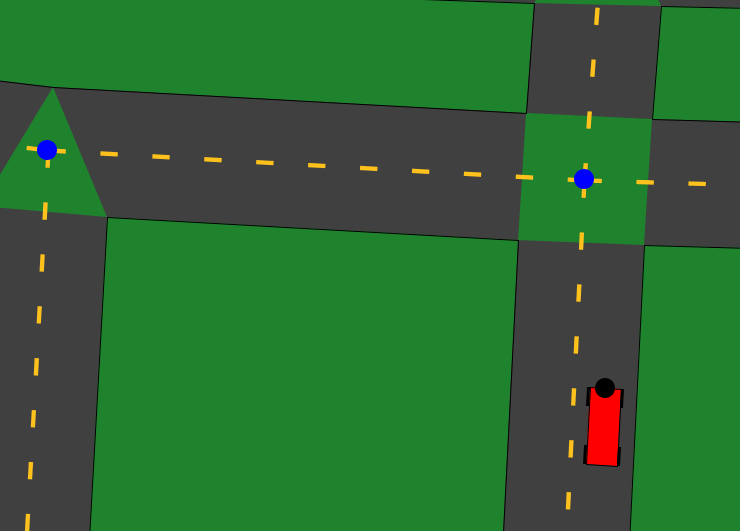
\includegraphics[width=0.5\textwidth]{astar}
  \end{center}
  \caption{$A^*$ navigation at work. The blue dots indicate the route.}
  \label{astar}
\end{figure}
We do deliberative navigation using the $A^*$ graph search algorithm,
which takes a heuristic function $h$ and finds a path between two
nodes on a graph. If $h$ satisfies certain properties, the path
returned will be optimal. We use the Euclidean distance formula
$h(n_1, n_2)=\sqrt{(n_1.x - n_2.x)^2 + (n_1.y - n_2.y)^2}$ which
satisfies these properties. The agent is modeled as a finite state
machine with four states: start, straight, turn, and replan. The agent
begins operation in the start state wherein it calculates the optimal
route to its destination. Once that is done, it begins traveling
forward until it is twice the road width from its starting node. It
then transitions to straight mode, where it ensures that its $\phi$ is
set parallel to the road. When it reaches a node, it pops the top node
off the route stack and enters turn mode. In turn mode it sets its
$\phi$ parallel to the vector between its target node (the node on the
top of the route stack) and itself. This ensures the agent stays on
the road at all times. Finally, when the agent has traveled past the
node, it reverts back to straight mode. If the agent reaches a node
which is not the next on its route, it enters replan mode, where it
immediately stops and calculates a new route to its destination from
its current position. Replanning can also be triggered by the server
sending a new destination.

\subsection{Reactive Agent}
\begin{figure}[h]
  \begin{center}
    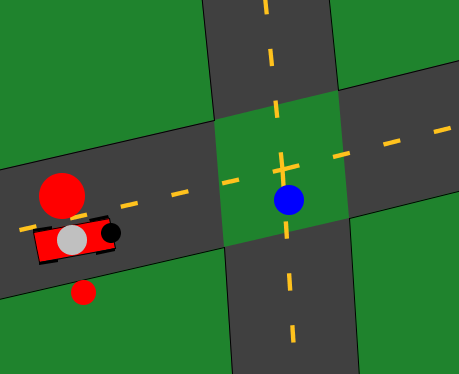
\includegraphics[width=0.5\textwidth]{dynamical}
  \end{center}
  \caption{Dynamical navigation at work. The red circles are obstacles
    that move along the road with the agent, while the blue circle is
    an intermediate target.}
  \label{dynamical}
\end{figure}


\subsection{Hybrid Agent}

\section{Results}

\section{Conclusion}
\subsection{Unreached goals}
- cached map rendering
- realistic choice variables

\end{document}
